\chapter{Measurements from IMU}\label{app:IMUMeasurementsAppendix}
\textbf{Name: Group 630}\\
\textbf{Date: 2/05 - 2016}

\subsubsection{Purpose}
Get data from the IMU and the potentiometer when running the state-space controller, and used it to design the complementary filter.             

\subsubsection{List of Equipment}
\begin{table}[H]
	\centering
	\begin{tabular}{|l|l|p{4.3cm}|}
		\hline%------------------------------------------------------------------------------------
		\textbf{Instrument}                        &  \textbf{AAU-no.}  &  \textbf{Type}       \\
		\hline%------------------------------------------------------------------------------------
		Dedicated Power Supply of Cubli \small{(24 V - 3 A)} &               &  XP Power, AEB70US24 \\
		\hline%------------------------------------------------------------------------------------
		Computer                &              &  Asus A55V          \\
		\hline%------------------------------------------------------------------------------------
	\end{tabular}
\end{table}
\subsubsection{Procedure}
\begin{enumerate}
	  \item Plug the power supply given of the Cubli.
	  \item Wait until the blue LEDs on the Beaglebone Black start blinking slowly and connect the USB cable to the PC.
	  \item Send the binary compiled program of the controller to the board.
	  \item Connect to a distant terminal on the Beaglebone Black through SSH and launch the program.
	  \item Let the program run with the state-space controller.
	  \item Apply small disturbances to the Cubli so there is some variations in the angle
	  \item Stop the program (by pressing \textit{Q} and \textit{ENTER}).
	  \item Retrieve the log file from the Cubli setup with the recorded data.
\end{enumerate}

\subsubsection{Results}

\begin{figure}[H]
	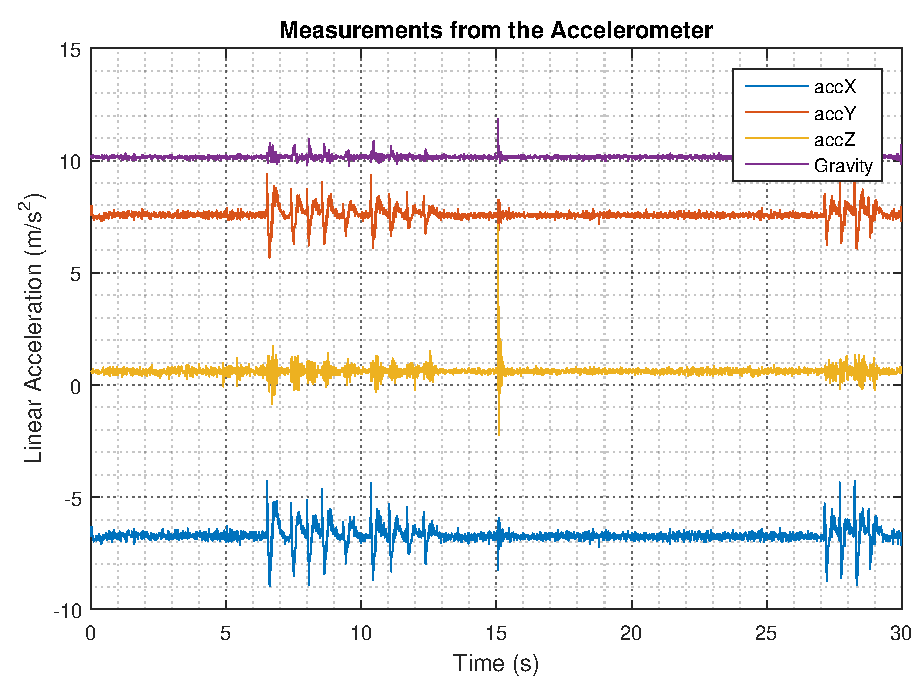
\includegraphics[scale=.75]{figures/accData}
	\centering
	\caption{Linear acceleration measurements from the accelerometer and the calculated gravity magnitude}
\end{figure} \label{accData}
%
\begin{figure}[H]
	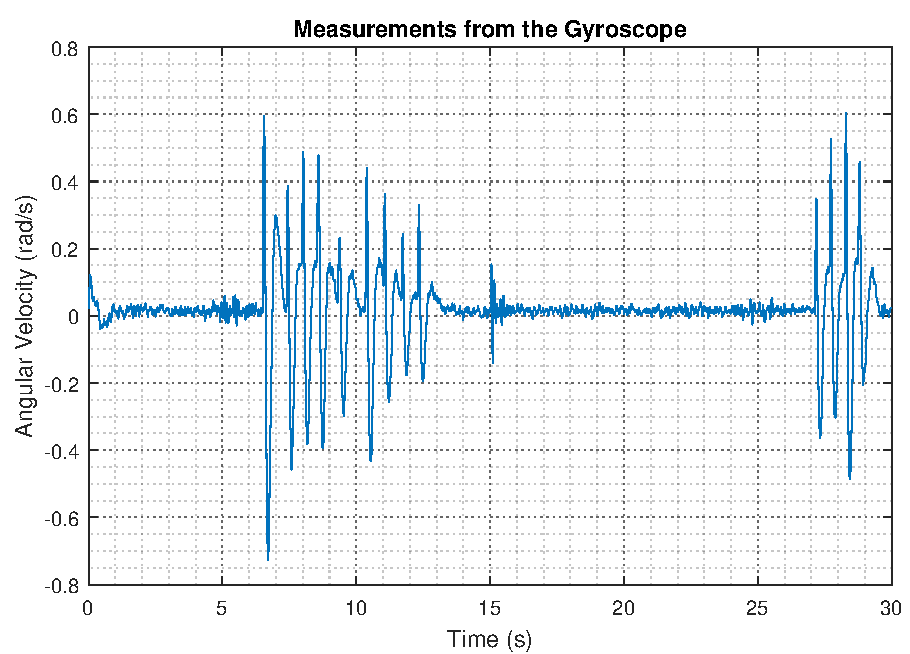
\includegraphics[scale=.75]{figures/gyroData}
	\centering
	\caption{Angular velocity measurements from the gyroscope}
\end{figure} \label{gyroData}
%
\begin{figure}[H]
	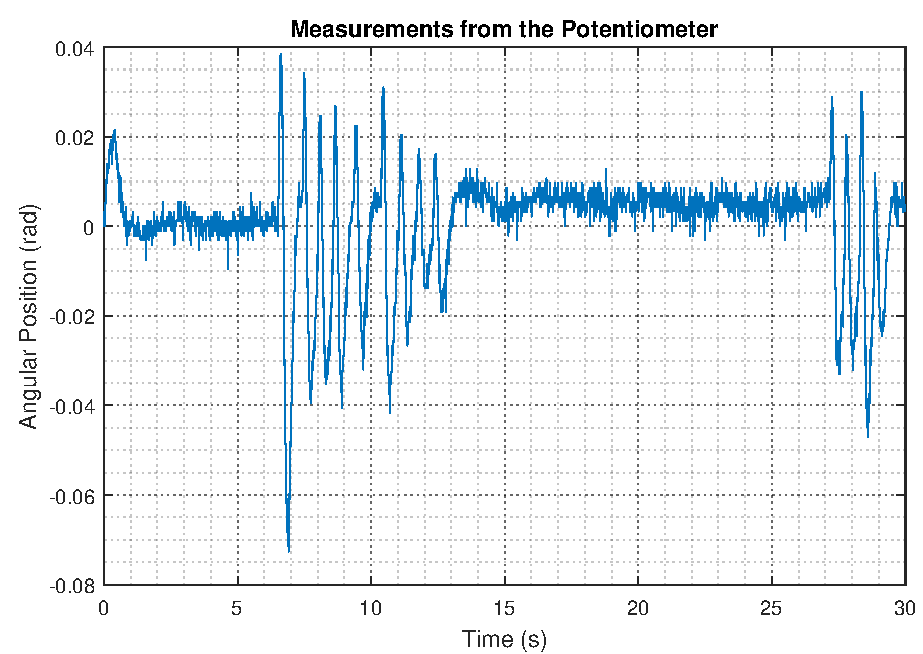
\includegraphics[scale=.75]{figures/potData}
	\centering
	\caption{Angle measurements from the potentiometer}
\end{figure} \label{potData}
